

\tikzset{every picture/.style={line width=0.75pt}} %set default line width to 0.75pt        

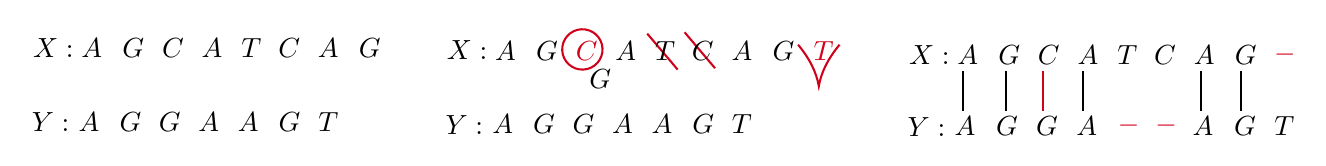
\begin{tikzpicture}[x=0.5pt,y=0.5pt,yscale=-1,xscale=1]
%uncomment if require: \path (0,146); %set diagram left start at 0, and has height of 146

%Straight Lines [id:da20102540282157666] 
\draw [color={rgb, 255:red, 208; green, 2; blue, 27 }  ,draw opacity=1 ]   (490,12) -- (512,38) ;
%Straight Lines [id:da009710943404266925] 
\draw [color={rgb, 255:red, 208; green, 2; blue, 27 }  ,draw opacity=1 ]   (463,13) -- (485,39) ;
%Shape: Circle [id:dp011981877187195566] 
\draw  [color={rgb, 255:red, 208; green, 2; blue, 27 }  ,draw opacity=1 ] (401.56,25.14) .. controls (401.15,17.1) and (407.35,10.25) .. (415.39,9.85) .. controls (423.43,9.45) and (430.28,15.64) .. (430.68,23.68) .. controls (431.09,31.73) and (424.89,38.57) .. (416.85,38.98) .. controls (408.81,39.38) and (401.96,33.19) .. (401.56,25.14) -- cycle ;
\draw  [color={rgb, 255:red, 208; green, 2; blue, 27 }  ,draw opacity=1 ] (602,21) .. controls (593.67,31) and (588.67,41) .. (587,51) .. controls (585.33,41) and (580.33,31) .. (572,21) ;
%Straight Lines [id:da5184853822717996] 
\draw    (691,40) -- (691,69) ;
%Straight Lines [id:da3211316725378842] 
\draw    (722,40) -- (722,69) ;
%Straight Lines [id:da18937901909445498] 
\draw [color={rgb, 255:red, 208; green, 2; blue, 27 }  ,draw opacity=1 ]   (749,40) -- (749,69) ;
%Straight Lines [id:da5526061509479675] 
\draw    (778,40) -- (778,69) ;
%Straight Lines [id:da6049458027827691] 
\draw    (863,40) -- (863,69) ;
%Straight Lines [id:da591487642150084] 
\draw    (892,40) -- (892,69) ;

% Text Node
\draw (81.5,14.5) node [anchor=north west][inner sep=0.75pt]   [align=left] {$\displaystyle G$};
% Text Node
\draw (167.45,14.5) node [anchor=north west][inner sep=0.75pt]   [align=left] {$\displaystyle \textcolor[rgb]{0,0,0}{T}$};
% Text Node
\draw (110.15,14.5) node [anchor=north west][inner sep=0.75pt]   [align=left] {$\displaystyle C$};
% Text Node
\draw (222.75,14.5) node [anchor=north west][inner sep=0.75pt]   [align=left] {$\displaystyle A$};
% Text Node
\draw (252.42,14.5) node [anchor=north west][inner sep=0.75pt]   [align=left] {$\displaystyle G$};
% Text Node
\draw (138.8,14.5) node [anchor=north west][inner sep=0.75pt]   [align=left] {$\displaystyle A$};
% Text Node
\draw (79.37,67.5) node [anchor=north west][inner sep=0.75pt]   [align=left] {$\displaystyle G$};
% Text Node
\draw (107.89,67.5) node [anchor=north west][inner sep=0.75pt]   [align=left] {$\displaystyle G$};
% Text Node
\draw (164.93,67.5) node [anchor=north west][inner sep=0.75pt]   [align=left] {$\displaystyle A$};
% Text Node
\draw (194.45,67.5) node [anchor=north west][inner sep=0.75pt]   [align=left] {$\displaystyle G$};
% Text Node
\draw (136.41,67.5) node [anchor=north west][inner sep=0.75pt]   [align=left] {$\displaystyle A$};
% Text Node
\draw (223,67.5) node [anchor=north west][inner sep=0.75pt]   [align=left] {$\displaystyle T$};
% Text Node
\draw (51.85,14.5) node [anchor=north west][inner sep=0.75pt]   [align=left] {$\displaystyle A$};
% Text Node
\draw (49.85,67.5) node [anchor=north west][inner sep=0.75pt]   [align=left] {$\displaystyle A$};
% Text Node
\draw (194.1,14.5) node [anchor=north west][inner sep=0.75pt]   [align=left] {$\displaystyle C$};
% Text Node
\draw (17,14) node [anchor=north west][inner sep=0.75pt]   [align=left] {$\displaystyle X:$};
% Text Node
\draw (16,68) node [anchor=north west][inner sep=0.75pt]   [align=left] {$\displaystyle Y:$};
% Text Node
\draw (380.5,16.5) node [anchor=north west][inner sep=0.75pt]   [align=left] {$\displaystyle G$};
% Text Node
\draw (466.45,16.5) node [anchor=north west][inner sep=0.75pt]   [align=left] {$\displaystyle \textcolor[rgb]{0,0,0}{T}$};
% Text Node
\draw (409.15,16.5) node [anchor=north west][inner sep=0.75pt]   [align=left] {$\displaystyle \textcolor[rgb]{0.82,0.01,0.11}{C}$};
% Text Node
\draw (521.75,16.5) node [anchor=north west][inner sep=0.75pt]   [align=left] {$\displaystyle A$};
% Text Node
\draw (551.42,16.5) node [anchor=north west][inner sep=0.75pt]   [align=left] {$\displaystyle G$};
% Text Node
\draw (437.8,16.5) node [anchor=north west][inner sep=0.75pt]   [align=left] {$\displaystyle A$};
% Text Node
\draw (378.37,69.5) node [anchor=north west][inner sep=0.75pt]   [align=left] {$\displaystyle G$};
% Text Node
\draw (406.89,69.5) node [anchor=north west][inner sep=0.75pt]   [align=left] {$\displaystyle G$};
% Text Node
\draw (463.93,69.5) node [anchor=north west][inner sep=0.75pt]   [align=left] {$\displaystyle A$};
% Text Node
\draw (493.45,69.5) node [anchor=north west][inner sep=0.75pt]   [align=left] {$\displaystyle G$};
% Text Node
\draw (435.41,69.5) node [anchor=north west][inner sep=0.75pt]   [align=left] {$\displaystyle A$};
% Text Node
\draw (522,69.5) node [anchor=north west][inner sep=0.75pt]   [align=left] {$\displaystyle T$};
% Text Node
\draw (350.85,16.5) node [anchor=north west][inner sep=0.75pt]   [align=left] {$\displaystyle A$};
% Text Node
\draw (348.85,69.5) node [anchor=north west][inner sep=0.75pt]   [align=left] {$\displaystyle A$};
% Text Node
\draw (493.1,16.5) node [anchor=north west][inner sep=0.75pt]   [align=left] {$\displaystyle C$};
% Text Node
\draw (316,16) node [anchor=north west][inner sep=0.75pt]   [align=left] {$\displaystyle X:$};
% Text Node
\draw (315,70) node [anchor=north west][inner sep=0.75pt]   [align=left] {$\displaystyle Y:$};
% Text Node
\draw (418.89,36.5) node [anchor=north west][inner sep=0.75pt]   [align=left] {$\displaystyle G$};
% Text Node
\draw (581,16.5) node [anchor=north west][inner sep=0.75pt]   [align=left] {$\displaystyle \textcolor[rgb]{0.82,0.01,0.11}{T}$};
% Text Node
\draw (714.5,19.25) node [anchor=north west][inner sep=0.75pt]   [align=left] {$\displaystyle G$};
% Text Node
\draw (800.45,19.25) node [anchor=north west][inner sep=0.75pt]   [align=left] {$\displaystyle \textcolor[rgb]{0,0,0}{T}$};
% Text Node
\draw (743.15,19.25) node [anchor=north west][inner sep=0.75pt]   [align=left] {$\displaystyle C$};
% Text Node
\draw (855.75,19.25) node [anchor=north west][inner sep=0.75pt]   [align=left] {$\displaystyle A$};
% Text Node
\draw (885.42,19.25) node [anchor=north west][inner sep=0.75pt]   [align=left] {$\displaystyle G$};
% Text Node
\draw (771.8,19.25) node [anchor=north west][inner sep=0.75pt]   [align=left] {$\displaystyle A$};
% Text Node
\draw (712.87,70.75) node [anchor=north west][inner sep=0.75pt]   [align=left] {$\displaystyle G$};
% Text Node
\draw (741.89,70.75) node [anchor=north west][inner sep=0.75pt]   [align=left] {$\displaystyle G$};
% Text Node
\draw (854.97,70.75) node [anchor=north west][inner sep=0.75pt]   [align=left] {$\displaystyle A$};
% Text Node
\draw (884.99,70.75) node [anchor=north west][inner sep=0.75pt]   [align=left] {$\displaystyle G$};
% Text Node
\draw (770.91,70.75) node [anchor=north west][inner sep=0.75pt]   [align=left] {$\displaystyle A$};
% Text Node
\draw (914,70.75) node [anchor=north west][inner sep=0.75pt]   [align=left] {$\displaystyle T$};
% Text Node
\draw (684.85,19.25) node [anchor=north west][inner sep=0.75pt]   [align=left] {$\displaystyle A$};
% Text Node
\draw (682.85,70.75) node [anchor=north west][inner sep=0.75pt]   [align=left] {$\displaystyle A$};
% Text Node
\draw (827.1,19.25) node [anchor=north west][inner sep=0.75pt]   [align=left] {$\displaystyle C$};
% Text Node
\draw (650,19.25) node [anchor=north west][inner sep=0.75pt]   [align=left] {$\displaystyle X:$};
% Text Node
\draw (649,71.25) node [anchor=north west][inner sep=0.75pt]   [align=left] {$\displaystyle Y:$};
% Text Node
\draw (800.93,70.75) node [anchor=north west][inner sep=0.75pt]   [align=left] {$\displaystyle \textcolor[rgb]{0.82,0.01,0.11}{-}$};
% Text Node
\draw (827.95,70.75) node [anchor=north west][inner sep=0.75pt]   [align=left] {$\displaystyle \textcolor[rgb]{0.82,0.01,0.11}{-}$};
% Text Node
\draw (913.89,19.25) node [anchor=north west][inner sep=0.75pt]   [align=left] {$\displaystyle \textcolor[rgb]{0.82,0.01,0.11}{-}$};


\end{tikzpicture}

